\section{持久与数据层}
\subsection{数据库}
本案选用 ProsgreSQL 作为数据库管理系统,PostgreSQL是开源的对象-关系数据库数据库管理系统,
在类似BSD许可与MIT许可的PostgreSQL许可下发行。本案的SQL结构设计如图\ref{erd}:

\begin{figure}[htbp!]
    \centering
    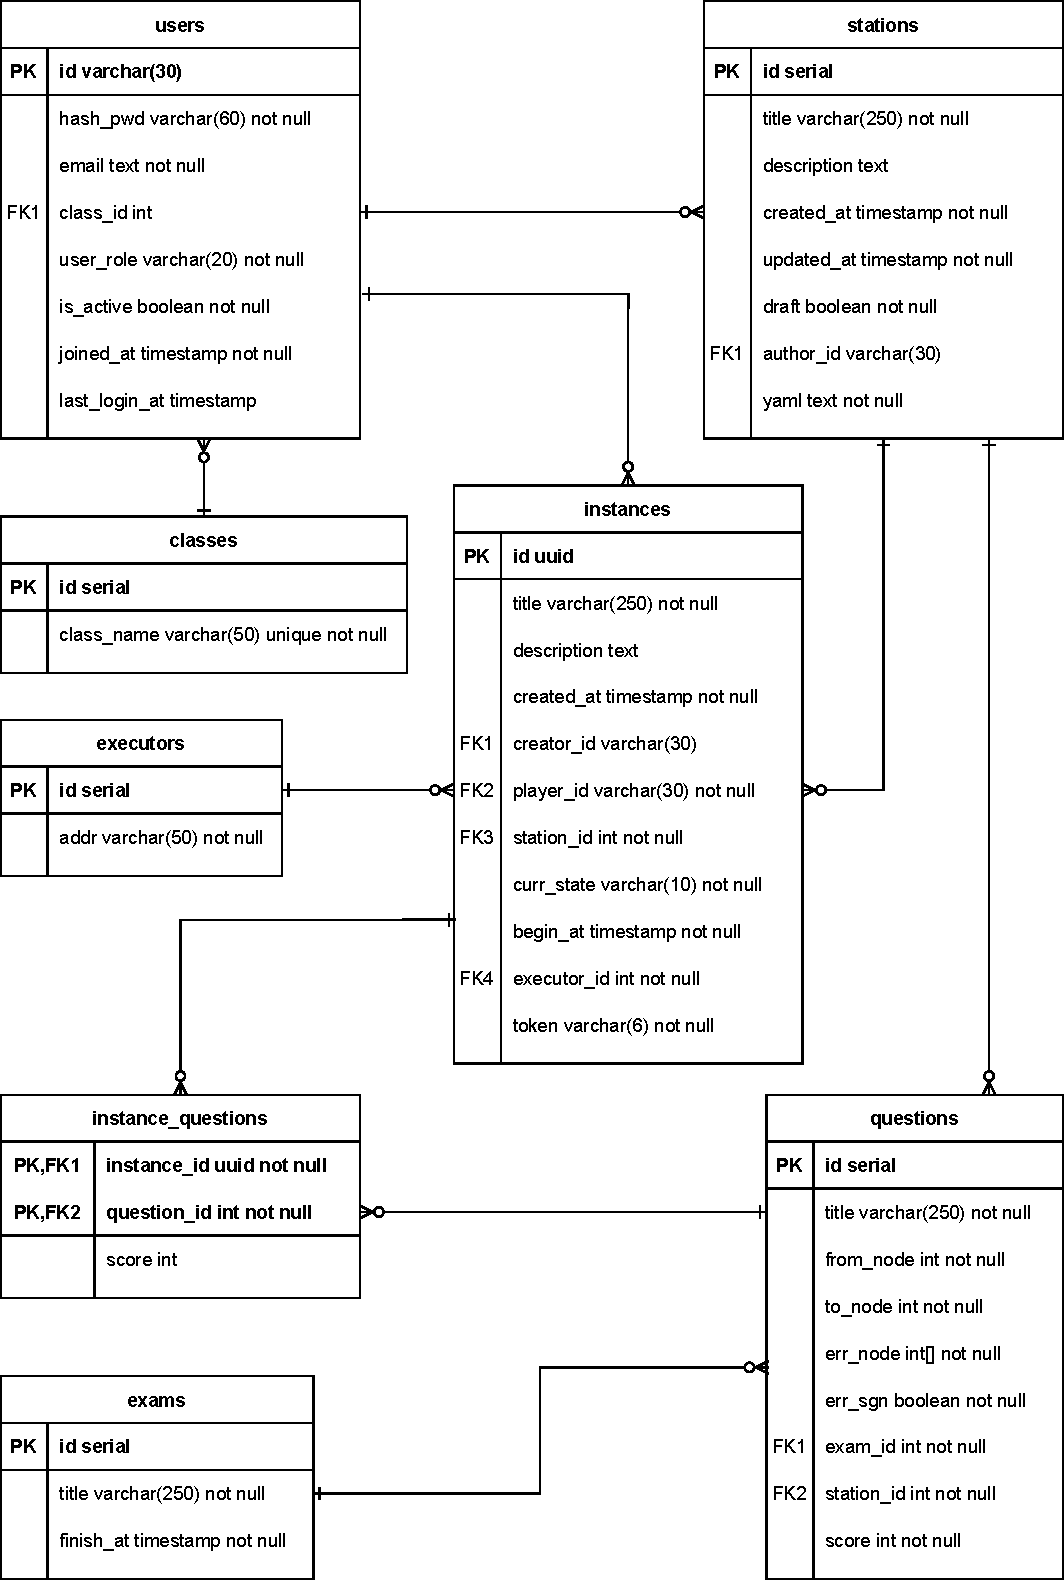
\includegraphics[width=0.95\textwidth]{figures/pdf/erd.pdf}
    \caption{\label{erd}数据库实体关系图}
\end{figure}

\subsubsection{表结构}

\paragraph 班级classes

\begin{lstlisting}
CREATE TABLE classes(
    id         serial       primary key,
    class_name varchar(50)  unique not null
)
\end{lstlisting}
主键id为自增整数,class\_name为班级名称

\paragraph 用户users

\begin{lstlisting}
CREATE TABLE users (
    id             varchar(30)     primary key,
    hash_pwd       varchar(60)     not null,
    email          text            not null,
    class_id       int  references classes(id) on delete set null,
    user_role      varchar(20)     not null,
    is_active      boolean         not null default 't',
    joined_at      timestamp       not null default now(),
    last_login_at  timestamp       default now()
)
\end{lstlisting}
解释:
\begin{itemize}
    \item 主键为id,类型为字符串,即用户自定义的用户id
    \item hash\_pwd 为加密后的用户密码
    \item email 为用户的电子邮箱地址
    \item class\_id 是表classes 的外键,表示用户所属的班级
    \item user\_role 表示用户角色
    \item is\_active 表示账户是否可用(未被禁用)
    \item joined\_at 和 last\_login\_at 默认是插入时的时间
\end{itemize}

\paragraph 车站stations

\begin{lstlisting}
CREATE TABLE stations (
    id          serial        primary key,
    title       varchar(250)  not null,
    description text,
    created_at  timestamp     not null default now(),
    updated_at  timestamp     not null default now(),
    draft       boolean       not null default 'f',
    author_id varchar(30) references users(id) on delete set null,
    yaml        text          not null
)
\end{lstlisting}
解释:
\begin{itemize}
    \item 主键为id, 自增整数
    \item title 为车站的标题
    \item description 为可空键,表示车站的备注
    \item draft 表示是否为草稿
    \item author\_id 是表 users 的外键,表示作者
    \item created\_at 和 updated\_at 默认是插入时的时间
    \item yaml 即为车站的描述文件内容
\end{itemize}

\paragraph 执行器executors

\begin{lstlisting}
CREATE TABLE executors (
    id             serial        primary key,
    addr           varchar(50)   not null
)
\end{lstlisting}
addr是该runtime的地址。

\paragraph 考试exams

\begin{lstlisting}
CREATE TABLE exams (
    id           serial        primary key,
    title        varchar(250)  not null,
    finish_at    timestamp     not null
)
\end{lstlisting}
finish\_at 表示结束时间,是考试特有的属性。

\paragraph 实例instances

\begin{lstlisting}
CREATE TABLE instances (
    id      uuid    primary key default gen_random_uuid(),
    title   varchar(250)  not null,
    description text,
    created_at  timestamp     not null  default now(),
    creator_id  varchar(30) references users(id) on delete ...,
    player_id   varchar(30)   not null  references users(id),    
    station_id  int           not null  references stations(id),
    curr_state  varchar(10)   not null,
    begin_at    timestamp     not null  default now(),
    executor_id int           not null  references executors(id),
    token       varchar(6)    not null
)
\end{lstlisting}
解释:
\begin{itemize}
    \item 主键为id, 类型是uuid
    \item title 为实例标题
    \item curr\_state 表示实例当前的状态
    \item creator\_id 是表 users 的外键,表示创建者
    \item player\_id 是表 users 的外键,表示实例的用户
    \item created\_at  默认是插入时的时间
    \item begin\_at 表示实例的开始时间
    \item executor\_id 表示该实例的运行时id,是executors表的外键
    \item station\_id 是表 stations 的外键,表示实例的车站
    \item token 是游客令牌
\end{itemize}

\paragraph 问题questions

\begin{lstlisting}
CREATE TABLE questions (
    id          serial        primary key,
    title       varchar(250)  not null,
    from_node   int           not null,
    to_node     int           not null,
    err_node    int[]         not null,
    err_sgn     boolean       not null,
    exam_id     int           not null  references exams(id),
    station_id  int           not null  references stations(id),
    score       int           not null
)
\end{lstlisting}
解释:
\begin{itemize}
    \item from\_node 是本题目进路自何处
    \item to\_node 是本题目进路往何处
    \item err\_node 是本题目的预设故障结点
    \item err\_dgn 是本题目进路信号机是否出错
    \item exam\_id 是表 exams 的外键,表示本题目属于哪个考试
    \item station\_id 是表 stations 的外键,表示本题目属于哪个车站
    \item score 表示本道题赋分几何
\end{itemize}

\paragraph 实例问题(即“考题”)instance\_questions

\begin{lstlisting}
CREATE TABLE instance_questions (
    instance_id    uuid   not null references instances(id),
    question_id    int    not null references questions(id),
    score          int,
    PRIMARY KEY (instance_id, question_id)
)
\end{lstlisting}

本表使用instance\_id和question\_id两个外键作为联合主键,本表的一个记录表示
某个实例(必然为考试实例)的某个题目得分几何。score是可空的,因为在新建考试实例的
时候就会在本表中新建进路,在完成某道考题的时候更新记录。

\subsection{持久层}
\subsubsection{ORM}
本案采用ORM以提升开发效率,ORM 是一种程序设计技术,用于将数据库的记录映射到程序语言的对象中,
或者将对象映射到某个表中,其封装了CRUD的SQL语句操作,可以让开发者从表中直接读入一个对象。或者将
一个对象插入某个表。效果上说,它其实是创建了一个可在编程语言里使用的“虚拟对象数据库”。

在本案的持久层 uroj-db 中,定义了程序的DAO层逻辑,封装了所有项目需要的数据库访问方法。
以便供Api, Auth, Executor 等服务复用。uroj采用diesel作为本案的ORM库,
将DAO层的各种结构体定义和上小结所定义的SQL表映射起来的,
就是diesel client所生成的schema。

这里简单介绍一下 diesel 的使用步骤。首先需要定义migration,migration可以简单理解为创建和删除表
的sql文件。将上一节的表定义好后。使用diesel生成schema,schema是diesel使用
rust macro定义的一些字段。之后我们需要定义DAO层的struct,对于一个表一般而言需要两种
struct,一个是读取用一个是插入用,但需要derive diesel提供的相应的过程宏,这样就可以
将sql表和DAO 层 struct映射起来,再使用diesel提供的方法进行CRUD操作。

\subsubsection{连接池}
连接池(英语:connection pool)是维护的数据库连接的缓存,
以便在将来需要对数据库发出请求时可以重用连接。
每次需要再打开一个新的数据库连接都是低效的,而且在高流量条件下会导致资源耗尽。
可以使用连接池解决这个问题以提高在数据库上执行命令的性能。
为每个用户打开和维护数据库连接,尤其是对动态数据库驱动的网站应用程序发出的请求,
既昂贵又浪费资源。在连接池中,创建连接之后,将连接放在池中并再次使用,这样就不必创建新的连接。
如果所有连接都正在使用,则创建一个新连接并将其添加到池中。
连接池还减少了用户必须等待创建与数据库的连接的时间。

uroj 采用 r2d2 作为数据库连接池,r2d2 是rust的一个通用连接池。
r2d2对于它所管理的连接类型是不可知的。
ManageConnection特性的实现者提供了数据库特定的逻辑来创建和检查连接的健康状况。

在 uroj-db crate 中使用如下create\_connection\_pool函数创建一个连接池。在
uroj-api 和 uroj-runtime 使用本函数创建连接池。
\begin{lstlisting}
use diesel::r2d2::{ConnectionManager, Pool};
use diesel::{pg::PgConnection, r2d2::PooledConnection};

pub type PgPool = Pool<ConnectionManager<PgConnection>>;
pub type Conn = PooledConnection<ConnectionManager<PgConnection>>;

pub fn create_connection_pool() -> PgPool {
    let url = env::var("DATABASE_URL").expect("Can't get DB URL");
    let manager = ConnectionManager::<PgConnection>::new(url);
    Pool::builder()
        .build(manager)
        .expect("Failed to create pool")
}
\end{lstlisting}